\documentclass[a4paper, 12pt]{report}
\usepackage[a4paper, %margenes de pagina
  left=2.5cm,
  right=2.5cm,
  top=1.5cm,
  bottom=2cm,
  includehead
]{geometry}
\usepackage[utf8]{inputenc}
%\usepackage[spanish]{babel} % Configuración de idioma
\usepackage{fancyhdr}
\usepackage{etoolbox}
\usepackage{titlesec}
\usepackage{titling} % para personalizar el título
\usepackage{tikz}
\usepackage{pgf}
\usetikzlibrary{positioning}
\UseRawInputEncoding
\usepackage{enumitem}

\usepackage{minted}
\setminted{
    linenos,          % Activa la numeración de líneas
    frame=single,      % Opcional: agrega un marco al código
    framesep=2mm,     % Opcional: separación entre el marco y el texto
    fontsize=\scriptsize,   % Opcional: cambia el tamaño de la fuente
    breaklines,
    encoding=utf8
}

\pagestyle{fancy}
\pagestyle{fancy}
\lhead{UTN-FRC}
\chead{Informática II}
\rhead{2R3}
\cfoot{\thepage}
\setlength{\headwidth}{\textwidth} % Hace que el ancho del encabezado coincida con el ancho del texto
\setlength{\headheight}{10pt}  % Ajusta la altura del encabezado
\setlength{\headsep}{20pt}     % Ajusta la separación entre el encabezado y el contenido
\patchcmd{\chapter}{\thispagestyle{plain}}{\thispagestyle{fancy}}{}{}

\DeclareMathSizes{12}{13}{6}{5}


\title{%
  \fontsize{25}{0}\selectfont Universidad Tecnológica Nacional \\
  \fontsize{22}{30}\selectfont Informática 2 \\
  \fontsize{18}{25}\selectfont SAPEI\\
  \fontsize{16}{20}\selectfont Sistema Alternativo de Pago para el Estacionamiento Institucional\\
}
\author{
Cortesini Luciano - 402719\\
Gil Ignacio - 401891\\
Grasso Gaston - 401892\\
Noccetti Santino - 405947 \\
Palombo Franco - 401910
}

\date{19 / 11 / 2024}

\titleformat{\chapter}[block]
  {\normalfont\huge\bfseries}{}{0pt}{\Huge}
\titlespacing*{\chapter}{0pt}{-30pt}{20pt}

% Redefinir el formato de las secciones para que solo muestren el título
\titleformat{\section}[block]
  {\normalfont\Large\bfseries}{}{0pt}{\Large}
\titlespacing*{\section}{0pt}{3.5ex plus 1ex minus .2ex}{2.3ex plus .2ex}

% Redefinir el formato de las subsecciones para que solo muestren el título
\titleformat{\subsection}[block]
  {\normalfont\large\bfseries}{}{0pt}{\large}
\titlespacing*{\subsection}{0pt}{3.25ex plus 1ex minus .2ex}{1.5ex plus .2ex}


\begin{document}
\maketitle
\section{Motivación}
    El tránsito en los alrededores de la Universidad Tecnológica Nacional, Facultad Regional Córdoba, es algo que es
    imposible de resolver, en especial en horas pico, o de cambio de turno. Ya habiendo asistido durante dos años
    consecutivos a cursar la carrera de ingeniería electrónica, uno empieza a prestarle atención al detalle de los
    eventos del día a día mientras estamos presentes en la facultad.

    Algo que como grupo hemos experimentado todos, es el tránsito que hay en las zonas circundantes a los ingresos
    para vehículos de la facultad. Es algo que se puede percibir siendo usuario del transporte público, peatón o
    conductor, ya que frenan todo. Este tránsito es perjudicial para todo aquel que quiera circular por cualquiera
    de las vías a las que se conecten los ingresos para vehículos.

\section{Definición del problema}
    Como se mencionó previamente, el problema está en el tránsito generado por los vehículos. Este tránsito (en gran
    parte) es generado por la fila de autos que hay en el ingreso al estacionamiento de la facultad, lo que obstruye
    la vía pública, reduciendo el flujo de vehículos y produciendo embotellamientos. La razón por la cual se genera la
    fila de autos, es por la lentitud del sistema de ingreso al estacionamiento. Este sistema requiere de un operario
    que ingrese la patente del vehículo de manera manual, el cual procede a generar un ticket de ingreso, y
    automáticamente se le descuenta el monto correspondiente al usuario.

\section{Solución propuesta}
    La alternativa que planteamos como solución, consta de un sistema Contactless, en el cual el usuario tiene en su
    posesión una tarjeta RFID, emitida por la entidad correspondiente, la cual tiene la identificación del mismo
    usuario. De este modo, no es necesario que el operario tenga que ingresar la patente del vehículo manualmente para
    poder generar el ticket, ya que el mismo no tiene razón de ser creado, debido a que para el ingreso o el egreso,
    se utiliza la tarjeta RFID. De tal forma, se puede mantener el conteo de vehículos en el estacionamiento, y además,
    se evita desperdiciar papel que se emite y se desecha en el mismo día.

\section{Objetivos}
    \begin{itemize}
        \item Ahorrar tiempo en el ingreso al estacionamiento de la institucion.
        \item Proveer una interfaz de usuario para el operario con herramientas de edicion e insercion de clientes.
        \item Almacenar eficientemente los datos de los clientes de manera local.
        \item Lograr un intercambio de información bidireccional entre dos arquitecturas. En este caso el entre el PC
            con linux y un arduino nano.
        \item Llevar a cabo la construccion de un prototipo del hardware.
    \end{itemize}

\newpage
\section{Planificación}
    Para poder llevar a cabo esta idea, empezamos por la organización de la misma y las necesidades o posibles
    problemas del proyecto. Decidimos usar Github y su sistema de control de versiones
    creando así los repositorios necesarios para distribuir de forma efectiva las partes de trabajo y así el proyecto
    pueda avanzar en simultaneo, permitiendo que algunos integrantes se centren en avanzar en partes especificas
    del proyecto, sin interferir en los avances del resto de los integrantes. Ademas, esta separación, permitió que
    los problemas se mantengan aislados, por repositorio, evitando así la cruza de errores y fallas, y mejorar el
    mantenimiento del código.

\section{Partes del Proyecto}
    La distribución de repositorios, y la distribución de trabajos, se realizo teniendo en cuenta las habilidades de
    cada uno de los integrantes. Las partes del proyecto y sus requisitos son los siguientes:
    \begin{enumerate}
        \item Hardware: Desarrollar el terminal SAPEI, montarlo en una protoboard y verificar la integridad y robustez
            del mismo.
        \item Firmware: Desarrollar el firmware para el terminal SAPEI, administrar el GPIO por medio de registros,
            emplear interrupciones y crear un protocolo de comunicación e inicialización del terminal SAPEI.
        \item Core: Desarrollar herramientas de uso general que sirven para todas las partes del proyecto.
        \item Client: Desarrollar una interfaz de usuario que interactúe de manera directa con el terminal y el Core,
            para administrar clientes, vehículos, carga de saldo y edición de propiedades.
    \end{enumerate}

\newpage
\section{Hardware}
    Los componentes usados para el hardware fueron:
    \begin{enumerate}
        \item Arduino Nano
        \item RC522 (Modulo RFID)
        \item transistor NPN BC548
        \item 3 Leds
        \item Buzzer Activo
        \item Protoboard
        \item Resistencias y cables
    \end{enumerate}

\section{Diagrama Funcional}
    \begin{figure}[h]
        \centering
        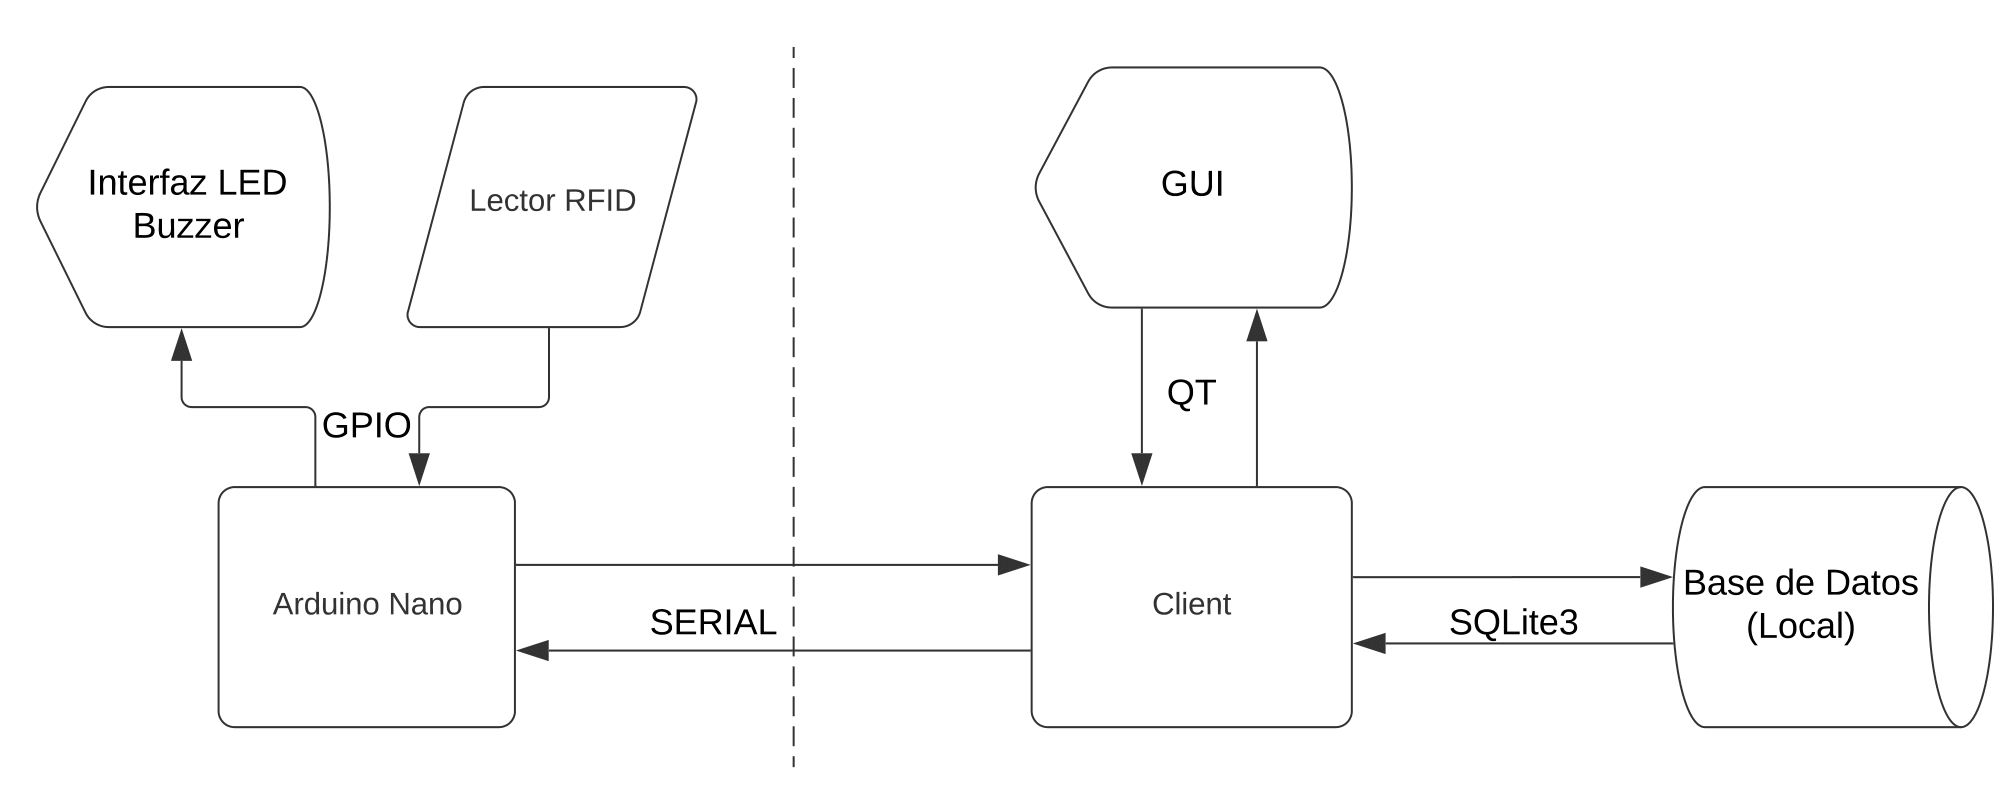
\includegraphics[width=1\textwidth]{./image1.png}
    \end{figure}

\section{Programa}
    El programa tiene una interfaz de usuario simple pero potente. Este programa es el encargado de administrar todos
    los clientes, comunicarse con la terminal SAPEI para leer las tarjetas y enviar códigos de estado al cliente.

    La interfaz esta compuesta por una sección de acciones, una ventana de estado, y una ventana de registro de
    operaciones.

    Ademas de poder agregar clientes, el operario puede editarlos, agregarle o borrarle vehículos e incluso borrar
    clientes.

\newpage
\section{Planes a futuro}
    El proyecto al principio tenia como objetivo tener un sistema descentralizado de almacenamiento de datos, como un
    servidor, por el cual se comunica con todos los clientes por el protocolo HTTP. Esto permite que en la facultad,
    haya múltiples terminales de acceso, pudiendo tener múltiples accesos a la facultad, y proveer de puestos
    exclusivos para la carga de saldo y creación de clientes.

    Debido a la escala del proyecto, no fue posible realizarlo, debido a que requería no solo desarrollar nuevas
    herramientas de uso común en el core, si no que también requería una reescritura y reestructuración completa del
    código en el Cliente, debido a que pasaba de ser administrador de la base de datos a un simple "endopoint" del
    servidor, quien se convertiría en el único programa con acceso de escritura a la base de datos.

    Este es un diagrama de funcionamiento de lo que habíamos planeado
    \begin{figure}[h]
        \centering
        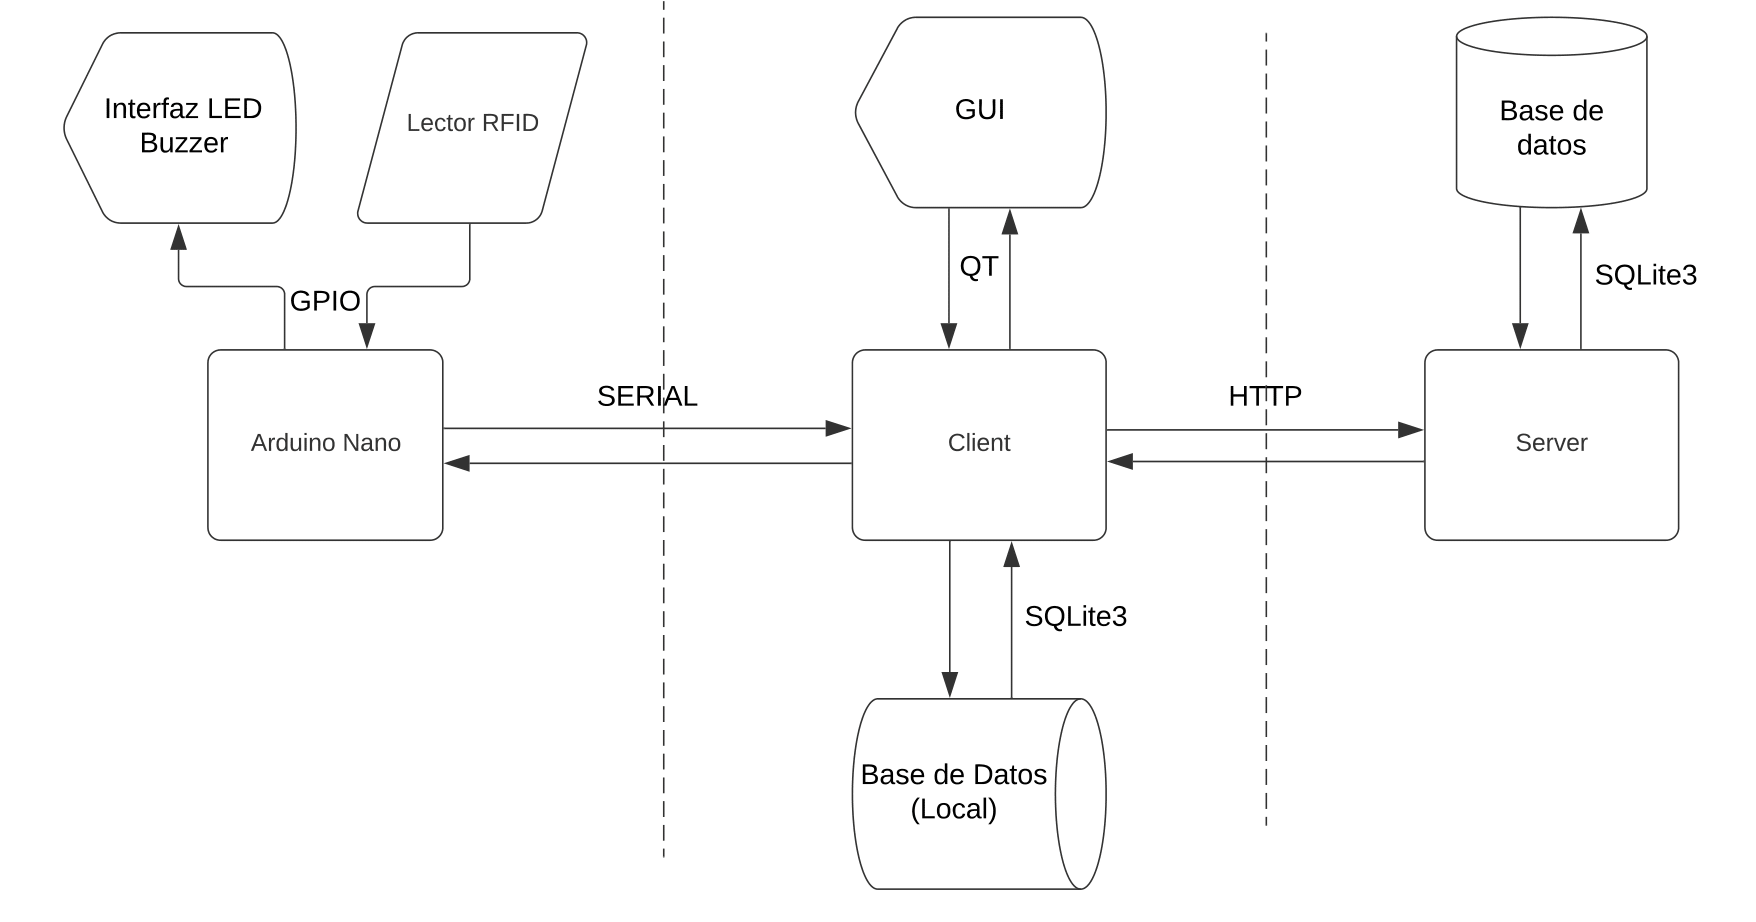
\includegraphics[width=1\textwidth]{./image2.png}
    \end{figure}

\newpage
\section{Firmware}
\begin{enumerate}[left=0pt]
    \item SAPEIFirwmare.ino
    \inputminted{c++}{../SAPEIFirmware/SAPEIFirmware.ino}
    \newpage
    \item gpio.h:
    \inputminted{c++}{../SAPEIFirmware/src/lib/gpio.h}
    \item gpio.cpp:
    \inputminted{c++}{../SAPEIFirmware/src/lib/gpio.cpp}
\end{enumerate}

\newpage
\section{Core}
\begin{enumerate}[left=0pt]
    \item Client.h
    \inputminted{c++}{../SAPEICore/Client.h}
    \item Client.cpp
    \inputminted{c++}{../SAPEICore/Client.cpp}
    \newpage
    \item Vehicle.h
    \inputminted{c++}{../SAPEICore/Vehicle.h}
    \item Vehicle.cpp
    \inputminted{c++}{../SAPEICore/Vehicle.cpp}
    \newpage
    \item Person.h
    \inputminted{c++}{../SAPEICore/Person.h}
    \item Person.cpp
    \inputminted{c++}{../SAPEICore/Person.cpp}
    \newpage
    \item Error.h
    \inputminted{c++}{../SAPEICore/Error.h}
    \item Error.cpp
    \inputminted{c++}{../SAPEICore/Error.cpp}
    \newpage
    \item Database.h
    \inputminted{c++}{../SAPEICore/DataBase.h}
    \item Database.cpp
    \inputminted{c++}{../SAPEICore/DataBase.cpp}
\end{enumerate}

\newpage
\section{Client}
\begin{enumerate}[left=0pt]
    \item main.cpp
    \inputminted{c++}{../SAPEIClient/main.cpp}
    \newpage
    \item addcarddialog.h
    \inputminted{c++}{../SAPEIClient/addcarddialog.h}
    \item addcarddialog.cpp
    \inputminted{c++}{../SAPEIClient/addcarddialog.cpp}
    \newpage
    \item addvehicledialog.h
    \inputminted{c++}{../SAPEIClient/addvehicledialog.h}
    \item addvehicledialog.cpp
    \inputminted{c++}{../SAPEIClient/addvehicledialog.cpp}
    \newpage
    \item balancehandler.h
    \inputminted{c++}{../SAPEIClient/balancehandler.h}
    \item balancehandler.cpp
    \inputminted{c++}{../SAPEIClient/balancehandler.cpp}
    \newpage
    \item clientlistdialog.h
    \inputminted{c++}{../SAPEIClient/clientlistdialog.h}
    \item clientlistdialog.cpp
    \inputminted{c++}{../SAPEIClient/clientlistdialog.cpp}
    \newpage
    \item editclientdialog.h
    \inputminted{c++}{../SAPEIClient/editclientdialog.h}
    \item editclientdialog.cpp
    \inputminted{c++}{../SAPEIClient/editclientdialog.cpp}
    \newpage
    \item editvehicledialog.h
    \inputminted{c++}{../SAPEIClient/editvehicledialog.h}
    \item editvehicledialog.cpp
    \inputminted{c++}{../SAPEIClient/editvehicledialog.cpp}
    \newpage
    \item mainwindow.h
    \inputminted{c++}{../SAPEIClient/mainwindow.h}
    \item mainwindow.cpp
    \inputminted{c++}{../SAPEIClient/mainwindow.cpp}
    \newpage
    \item serialhandler.h
    \inputminted{c++}{../SAPEIClient/serialhandler.h}
    \item serialhandler.cpp
    \inputminted{c++}{../SAPEIClient/serialhandler.cpp}
    \newpage
    \item vehiclelistdialog.h
    \inputminted{c++}{../SAPEIClient/vehiclelistdialog.h}
    \item vehiclelistdialog.cpp
    \inputminted{c++}{../SAPEIClient/vehiclelistdialog.cpp}
\end{enumerate}

\newpage
\section{Conclusiones}
    El proyecto SAPEI (Sistema Alternativo de Pago para el Estacionamiento Institucional) ha logrado cumplir con éxito
    los objetivos planteados, demostrando en el hipotetico caso de ser aplicada, ser una solución eficiente y práctica
    para abordar los problemas relacionados con el tiempo de ingreso vehicular al estacionamiento de la institución.
    A continuación, se destacan los principales logros obtenidos:
    \begin{itemize}
        \item Reducción del tiempo de ingreso al estacionamiento: La implementación del sistema basado en tarjetas RFID
          eliminó la necesidad de ingreso manual de datos por parte de un operario, acelerando significativamente el
          proceso de entrada y salida de vehículos.

        \item Desarrollo de una interfaz de usuario para el operario: Se diseñó y desarrolló una interfaz gráfica
          intuitiva y funcional, que permite a los operarios gestionar de manera eficiente la base de datos de clientes.
          Las herramientas de edición e inserción de clientes han facilitado la administración del sistema, optimizando
          el tiempo y esfuerzo requeridos para estas tareas.

        \item Almacenamiento eficiente de datos: La base de datos local implementada con SQLite garantizó un
          almacenamiento seguro y organizado de la información de los clientes y vehículos.

        \item Intercambio bidireccional de información entre arquitecturas: Se logró establecer una comunicación
          confiable y eficiente entre el Arduino Nano y el sistema operativo Linux en la PC. Este intercambio de datos
          en tiempo real permitió la integración armoniosa del hardware con la aplicación cliente, asegurando un
          funcionamiento fluido del sistema en su conjunto.

        \item Construcción de un prototipo funcional del hardware: El desarrollo y montaje del prototipo en una
          protoboard validó la viabilidad del sistema en un entorno físico. La integración de componentes como el
          módulo RFID, LEDs, y un buzzer permitió simular y probar el sistema completo, garantizando su correcto
          desempeño.
    \end{itemize}

    En resumen, el éxito del proyecto radica en la combinación efectiva de tecnologías de hardware y software para
    resolver un problema concreto de manera innovadora y sostenible. Los resultados obtenidos no solo cumplen con los
    objetivos iniciales, sino que también abren la puerta a futuras mejoras, como la expansión del sistema a múltiples
    terminales o la implementación de almacenamiento en la nube para una mayor escalabilidad.

\newpage
\section{Anexos}
    Repositorios de Github:
      \begin{figure}[H]
      \centering
      \begin{minipage}{0.3\textwidth}
        \centering
        
\includegraphics[width=1\textwidth]{./core.png}
        \textit{SAPEICore}
      \end{minipage}
      \hspace{0.5cm}
      \begin{minipage}{0.3\textwidth}
        \centering
        
\includegraphics[width=1\textwidth]{./client.png}
        \textit{SAPEIClient}
      \end{minipage}
      \hspace{0.5cm}
      \begin{minipage}{0.3\textwidth}
        \centering
        
\includegraphics[width=1\textwidth]{./firmware.png}
        \textit{SAPEIFirmware}
      \end{minipage}
    \end{figure}
\end{document}
